\documentclass[12pt]{article}
\usepackage{amsmath, amssymb}
\usepackage{tikz}
\usetikzlibrary{decorations.text}
\usepackage{pgfplots}
\usepackage{multicol}

\title{Introduction to\\
\textbf{Conic Sections}}\\
\author{Tutoring Centre Ferndale\\
\includegraphics[width=4em]{ApS_logo.png}}
\date{}

\begin{document}

\maketitle

Conic sections are the curves obtained by intersecting a plane with a point-to-point pair of cones. The type of curve formed depends on the angle at which the plane intersects the cone.\\\\

\includegraphics[width=\textwidth]{conic sections.png}

\newpage

\section*{Circle}
A circle is formed when the plane cuts the cone perpendicular to the cone's axis.

A circle is the set of all points in a plane that are equidistant from a given point called the centre.

\begin{itemize}
\item The distance from the center to any point on the circle is called the radius.
\item The distance across the circle passing through the centre is called the diameter.
\item The distance around the circle is called the circumference.
\item The ratio between the circumference and the diameter of a circle is $\pi$, the Greek letter Pi (equivalent to the English letter P,) which originally stood for perimeter. $\pi=\frac{\textrm{circumference}}{\textrm{diameter}}$.\\

\begin{minipage}{0.48\textwidth}
\centering
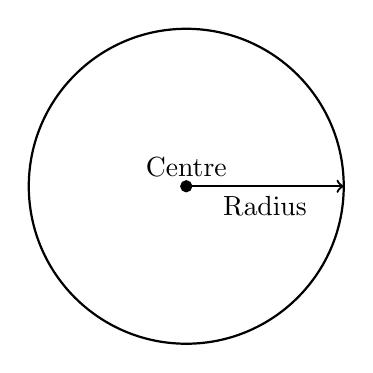
\begin{tikzpicture}
\draw[thick] (0,0) circle(2cm);
\filldraw[black] (0,0) circle(2pt) node[above] {Centre};
\draw[thick, ->] (0,0) -- (2,0) node[midway, below] {Radius};
\end{tikzpicture}
\end{minipage}
\hfill
\begin{minipage}{0.48\textwidth}
\centering
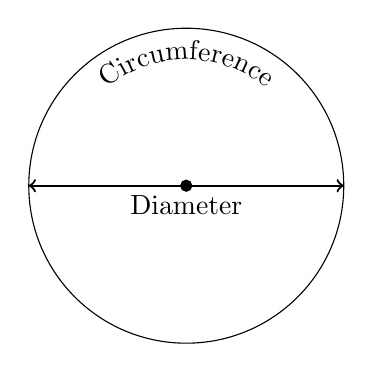
\begin{tikzpicture}
    \draw (0,0) circle [radius=2cm];
    \path[decorate,decoration={text along path, text={Circumference}, text align={align=center}}] 
        (-1.6,0) arc [start angle=180, end angle=0, radius=1.6cm];
    \filldraw[black] (0,0) circle(2pt);
    \draw[thick, <->] (-2,0) -- (2,0) node[midway, below] {Diameter};
\end{tikzpicture}
\end{minipage}

\item The equation of a circle is $x^2 + y^2 = r^2$, which is derived from Pythagoras' theorem.
\end{itemize}

\newpage

\section*{Ellipse}
An ellipse is formed when the plane cuts the cone at an angle to the axis, but the angle is less than the angle between the side of the cone and the axis. This results in a closed, oval shape.

\begin{itemize}
\item An ellipse is all points such that the sum of the distances from to two fixed points, called the foci, is constant.
\item For any point on the ellipse, the sum of the distances to the two foci is equal to the length of the major axis.

\begin{center}
\resizebox{0.5\textwidth}{!}{
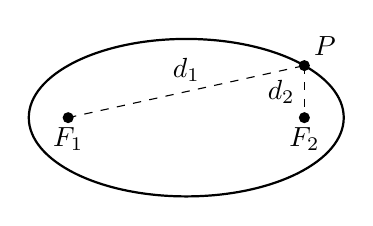
\begin{tikzpicture}
\draw[thick] (2,0) arc (0:360:2 and 1);
    \coordinate (F1) at (-1.5,0);
    \coordinate (F2) at (1.5,0);
    \fill (F1) circle (2pt) node[below] {$F_1$};
    \fill (F2) circle (2pt) node[below] {$F_2$};
    \coordinate (P) at (1.5, 0.6614);
    \fill (P) circle (2pt) node[above right] {$P$};
    \draw[dashed] (F1) -- (P) node[midway, above] {$d_1$};
    \draw[dashed] (P) -- (F2) node[midway, left] {$d_2$};
\end{tikzpicture}
}
\end{center}

\item The Equation for an ellipse is $\frac{x^2}{a^2} + \frac{y^2}{b^2} = 1$,
where \( a \) and \( b \) are the height and width of the ellipse.
\end{itemize}

\newpage

\section*{Parabola}
A parabola is formed when the plane is parallel to the slant of the cone, which is an angle equal to the angle between the side of the cone and the axis.

\begin{itemize}
\item Every point on a parabola is equally distant from a fixed point called the the focus and a central line called the directrix.\\

\begin{center}
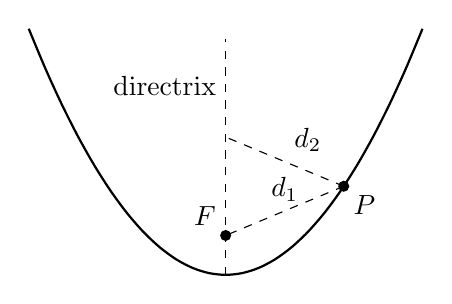
\begin{tikzpicture}
    \draw[thick, domain=-2.5:2.5, smooth, variable=\x] plot ({\x}, {0.5*\x*\x});
    \coordinate (F) at (0, 0.5);
    \fill (F) circle (2pt) node[above left] {$F$};
    \draw[dashed] (0,0) -- (0,3) node[pos=0.8,left] {directrix};
    \coordinate (P) at (1.5, 0.5*1.5^2);
    \fill (P) circle (2pt) node[below right] {$P$};
    \draw[dashed] (P) -- (F) node[midway, above] {$d_1$};
    \draw[dashed] (P) -- (0, 1.75) node[midway, above right] {$d_2$};
\end{tikzpicture}
\end{center}

\item Parabola is a Greek word which means "to place beside" or "comparison." The name comes from the way a parabola is the set of points equidistant from a focus and a directrix, the two distances being compared..
\item The equation of a parabola is $y = ax^2 + bx + c$.
\end{itemize}

\newpage

\section*{Hyperbola}
A hyperbola is formed when the plane cuts through both the upper and lower parts of the cone. This results in two separate, mirror-image curves.

\begin{itemize}
\item The difference in distances from any point on the hyperbola to the two foci is constant.

\begin{center}
\begin{tikzpicture}
    \draw[thick, domain=-3:3, smooth, variable=\x] plot ({\x}, {sqrt(1 + \x*\x)});
    \draw[thick, domain=-3:3, smooth, variable=\x] plot ({\x}, {-sqrt(1 + \x*\x)});
    \coordinate (F1) at (-2, 0);
    \coordinate (F2) at (2, 0);
    \fill (F1) circle (2pt) node[below] {$F_1$};
    \fill (F2) circle (2pt) node[below] {$F_2$};
\end{tikzpicture}
\end{center}

\item Hyperbola is a Greek word meaning "excess" or "overthrow." A hyperbola consists of two separate curves which are points where the difference in distances to the foci is constant. The excess is in relation to these distances.

\item The equation} of a hyperbola is $\frac{x^2}{a^2} - \frac{y^2}{b^2} = 1$, where \( a \) and \( b \) are related to the distances from the center to the vertices and foci.
\end{itemize}

\newpage

\section*{Degenerate Conic Sections}
These occur under special circumstances when the plane passes through the vertex of the cone.

Degenerate conic sections are called "degenerate" because they represent cases where the typical geometric properties of conic sections break down, leading to simpler or more limited forms. Unlike standard conic sections (circles, ellipses, parabolas, and hyperbolas), which are defined by their distinct shapes and properties, degenerate cases occur under specific conditions that result in a loss of the expected geometric structure.

\begin{itemize}
    \item \textbf{Point}:
    \begin{itemize}
        \item When the plane touches the vertex of the cone, and no part of the plane intersects the cone, the result is a single point.
        \end{itemize}
    
    \item \textbf{Line}:
    \begin{itemize}
        \item When the plane is tangent to the cone (only touching it at a single line), the result is a single line.
        \item It will be a linear equation of the form \( ax + by + c = 0 \).
    \end{itemize}
    
    \item \textbf{Pair of Intersecting Lines}:
    \begin{itemize}
        \item When the plane passes through the vertex and cuts the cone in two intersecting lines.
        \item This can occur in cases where the general quadratic equation is factorable into two linear equations.
    \end{itemize}
\end{itemize}

\end{document}
